\section*{Discussion}
The random forest parameters optimization could have been performed using a design of experiment instead. But this work focused more on the implementation of atlas-based segmentation methods.

The four atlas-based segmentation perform better with small brain parts, such as the amygdala, hippocampus and thalamus. This can be explained due to their relative static position and low distortion. 

For machine learning segmentation, grey and white matter have better results as atlas-based ones. Machine learning is able to interpret the subtle geometrical changes of those. This is clearly visible in the figure \ref{fig:compareGreyMatter}.

\begin{figure}[h!]
	\centering
	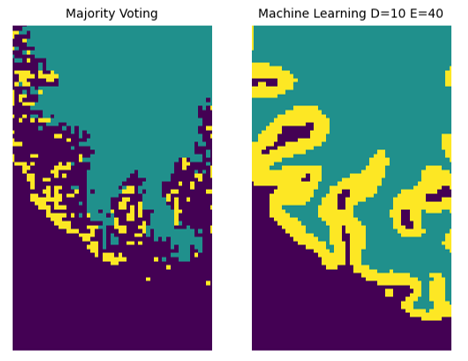
\includegraphics[width=.88\linewidth]{img/compareGreyMatter}
	\caption{Comparison between majority voting and machine learning segmentation for grey (yellow) and white matter (cyan).}
	\label{fig:compareGreyMatter}
\end{figure}

When comparing all four atlas-based segmentation algorithms, there is no major difference between majority voting, global weighted voting and shape based averaging. Local weighted voting significantly improves with grey and white matter, as seen in the results. The figure \ref{fig:compareSegmentationSlice} shows this case precisely. The edges of white matter and the grey matter are much more realistic and complete for the global weighted voting segmentation. The other three segmentations are very sparse at the frontier between grey and white matter.

\begin{figure}[h!]
	\centering
	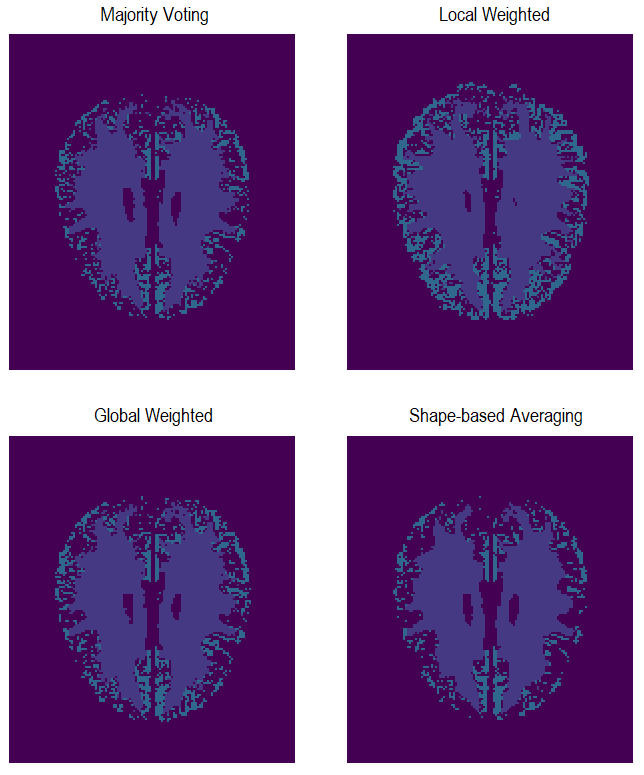
\includegraphics[width=.88\linewidth]{img/compareSegmentationSlice}
	\caption{Comparison between all 4 atlas-based segmentations for grey (cyan) and white matter (blue).}
	\label{fig:compareSegmentationSlice}
\end{figure}

Overall, the best performing algorithm of all those tested is the local weighted voting segmentation. The amygdala, hippocampus and thalamus have similar score as the other three atlas-based methods. The grey and white matter have a score close to the one with machine learning segmentation.